\documentclass[12pt,letterpaper]{article}

\usepackage[utf8]{inputenc}
\usepackage[spanish]{babel}
\usepackage{times}
\usepackage[left=3cm,top=2.5cm,bottom=2.5cm,right=2.5cm]{geometry}
\usepackage{graphicx}
\title{EV\_ 1\_ 6\_ Explicar\_ la\_ operación\_ de\_ los\_ circuitos\_ de\_ activación\_ con\_ tiristores\_ en\_ convertidores\_ CA-CD\_ y\_ CA-CA.}


\begin{document}
\maketitle




\paragraph{ UNIVERSIDAD POLITÉCNICA DE LA ZONA METROPOLITANA DE GUADALAJARA}

\
\begin{figure}[h!]
\begin{center}


\includegraphics[scale=0.8]{Upzmg.png} 
\label{Upzmg}


\end{center}
\end{figure}


\

\large{Perez de Alba Santiago Eduardo.\\
Fecha: 24 de septiembre del 2019.
\

Curso: Sep-Nov 2019.

\
Carrera: Ingeniería en Mecatronica.\

Docente: Moran Garabito Carlos Enrique}

\newpage

\section{Marco teórico:}
\

Un tiristor se comporta como un diodo cuando se aplica una corriente de puerta por el terminal. El proceso de activacion requiere que se cumplan dos condiciones:
	\
	1.- Debe aplicarse una intensidad de control en el terminal de puerta. Dicha intensidad debe tener condiciones de amplitud y duracion determinadas.
	\
	
	2.- En el momento de aplicar la intensidad de control en el terminal de puerta, la intensidad ánodo-cátodo debe ser positiva.

\

\begin{figure}[h!]
\begin{center}
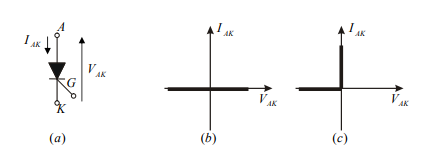
\includegraphics[width=8cm]{Tiristores.png} 
\caption{Figura 1. Símbolo y Curvas de un tiristor. (b) estado de bloqueo. (c) Estado de conducción}
\end{center}
\end{figure}

\

Una vez que un tiristor se ha activado y pasa a la condicion de conduccion, así permanece hasta que la intensidad del ánodo-cátodo se vuelven negativas. Esto hace que si la intensidad de ánodo-cátodo es tipo alterna, el tiristor conmuta automaticamente del estado de conduccion al de bloquea cada vez que dicha intensidad cambien de signo.
\

El tiristor permite un control externo de activacion, sin embargo, se desactiva automaticamente en las mismas condiciones en las que un diodo pasa a estado de bloqueo

\

\subsection{Puente de media onda: }
\

\

En el puente de media onda semi-controlado se puede sustituir el diodo por un tiristor el cual admite un control de conducción sencillo.
\

\begin{figure}[h!]
\begin{center}
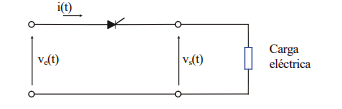
\includegraphics[width=8cm]{Medio puente-Semicontrolado.png} 
\caption{ Figura 2. Rectificador de media onda semicontrolado}
\end{center}


\end{figure}

\

\begin{figure}
\begin{center}
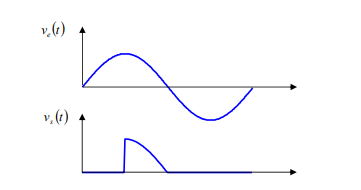
\includegraphics[scale=1]{Onda de tension entrada y salida.png} 
\caption{ Figura 3. Onda de tensiones de entrada y salida del rectificador.}

\end{center}


\end{figure}

\

\subsection*{Rectificador de media onda con carga resistiva-inductiva:}
\

Si el SCR es activado con cierto angulo $\alpha$ de retraso, la corriente incrementa lentamente debido al inductor. El voltaje en la carga es positivo y el inductor almacena energia mediante el campo magnetico. Sin embargo, cuando el semi-ciclo negativo desactiva al SCR, y el campo magnetico se descarga a través de la carga en sentido opuesto a su polaridad obteniendo el voltaje negativo

\

\subsection{Rectificador de onda completa controlado:}
\

Este circuito se basa en las leyes de Kirchoff debido a las mallas creadas por los tiristores, en el cual se demuestra que ambas parejas no pueden conducir al mismo tiempo, como tambien el voltaje inverso que soporta cada uno es igual al voltaje pico del generador.
Esto se da gracias a la siguiente formula:

$$ Vo=\frac{Vmax(1+\cos a)}{p}$$ 
\end{document}
